\documentclass[tikz,border=12pt]{standalone}
\usepackage{tikz}
\usepackage{amsmath}
\usepackage{amssymb}
\usetikzlibrary{
  shapes.geometric,
  shapes.multipart,
  arrows.meta,
  positioning,
  fit,
  backgrounds,
  shadows.blur,
  calc,
  matrix,
  decorations.pathreplacing,
  decorations.markings
}

%% ===== COLOR PALETTE =====
\definecolor{CPurple50}{HTML}{EEEDFE}
\definecolor{CPurple400}{HTML}{7D77D4}
\definecolor{CPurple600}{HTML}{534AB7}
\definecolor{CPurple800}{HTML}{3C3489}
\definecolor{CTeal50}{HTML}{E1F5EE}
\definecolor{CTeal400}{HTML}{3CB88A}
\definecolor{CTeal600}{HTML}{0F6E56}
\definecolor{CTeal800}{HTML}{085041}
\definecolor{CAmber50}{HTML}{FAEEDA}
\definecolor{CAmber400}{HTML}{D48B2E}
\definecolor{CAmber600}{HTML}{854F0B}
\definecolor{CCoral50}{HTML}{FAECE7}
\definecolor{CCoral400}{HTML}{D85A30}
\definecolor{CCoral600}{HTML}{993C1D}
\definecolor{CRed50}{HTML}{FCEBEB}
\definecolor{CRed400}{HTML}{C94040}
\definecolor{CRed600}{HTML}{A32D2D}
\definecolor{CGray50}{HTML}{F5F4F0}
\definecolor{CGray200}{HTML}{D8D5C8}
\definecolor{CGray500}{HTML}{888780}
\definecolor{CGray800}{HTML}{444441}
\definecolor{CBlue50}{HTML}{E6F1FB}
\definecolor{CBlue600}{HTML}{185FA5}
\definecolor{CWhite}{HTML}{FFFFFF}

%% ===== TIKZ STYLES =====
\tikzset{
  %% --- DFD nodes ---
  dfd process/.style={
    rectangle, rounded corners=6pt,
    draw, line width=0.8pt,
    text width=4.8cm, align=center,
    font=\small,
    inner sep=7pt, minimum height=1.1cm
  },
  dfd io/.style={
    rectangle, rounded corners=4pt,
    draw, line width=0.8pt,
    text width=9.6cm, align=center,
    font=\small,
    inner sep=7pt, minimum height=0.9cm
  },
  dfd cwe/.style={
    rectangle, rounded corners=3pt,
    text width=4.8cm, align=center,
    font=\scriptsize\bfseries,
    inner sep=4pt, minimum height=0.48cm
  },
  %% --- Arrows ---
  arr/.style={
    -Stealth, line width=0.9pt, color=CGray500
  },
  arr red/.style={
    -Stealth, line width=1.0pt, color=CRed400,
    dashed
  },
  arr teal/.style={
    -Stealth, line width=1.0pt, color=CTeal600
  },
  arr purple/.style={
    -Stealth, line width=1.0pt, color=CPurple600
  },
  arr amber/.style={
    -Stealth, line width=1.0pt, color=CAmber600
  },
  %% --- Labels ---
  edge label/.style={
    font=\scriptsize, text=CGray800,
    fill=CWhite, inner sep=2.5pt, rounded corners=2pt
  },
  title main/.style={font=\Large\bfseries, text=CGray800},
  title sub/.style={font=\small, text=CGray500},
  badge/.style={
    rectangle, rounded corners=2pt,
    font=\scriptsize\bfseries,
    inner sep=3.5pt, minimum height=0.48cm,
    text=CWhite
  }
}

\begin{document}
%% ===========================================================
%% DIAGRAM 3: SƠ ĐỒ LUỒNG DỮ LIỆU (DATA FLOW DIAGRAM)
%% ===========================================================
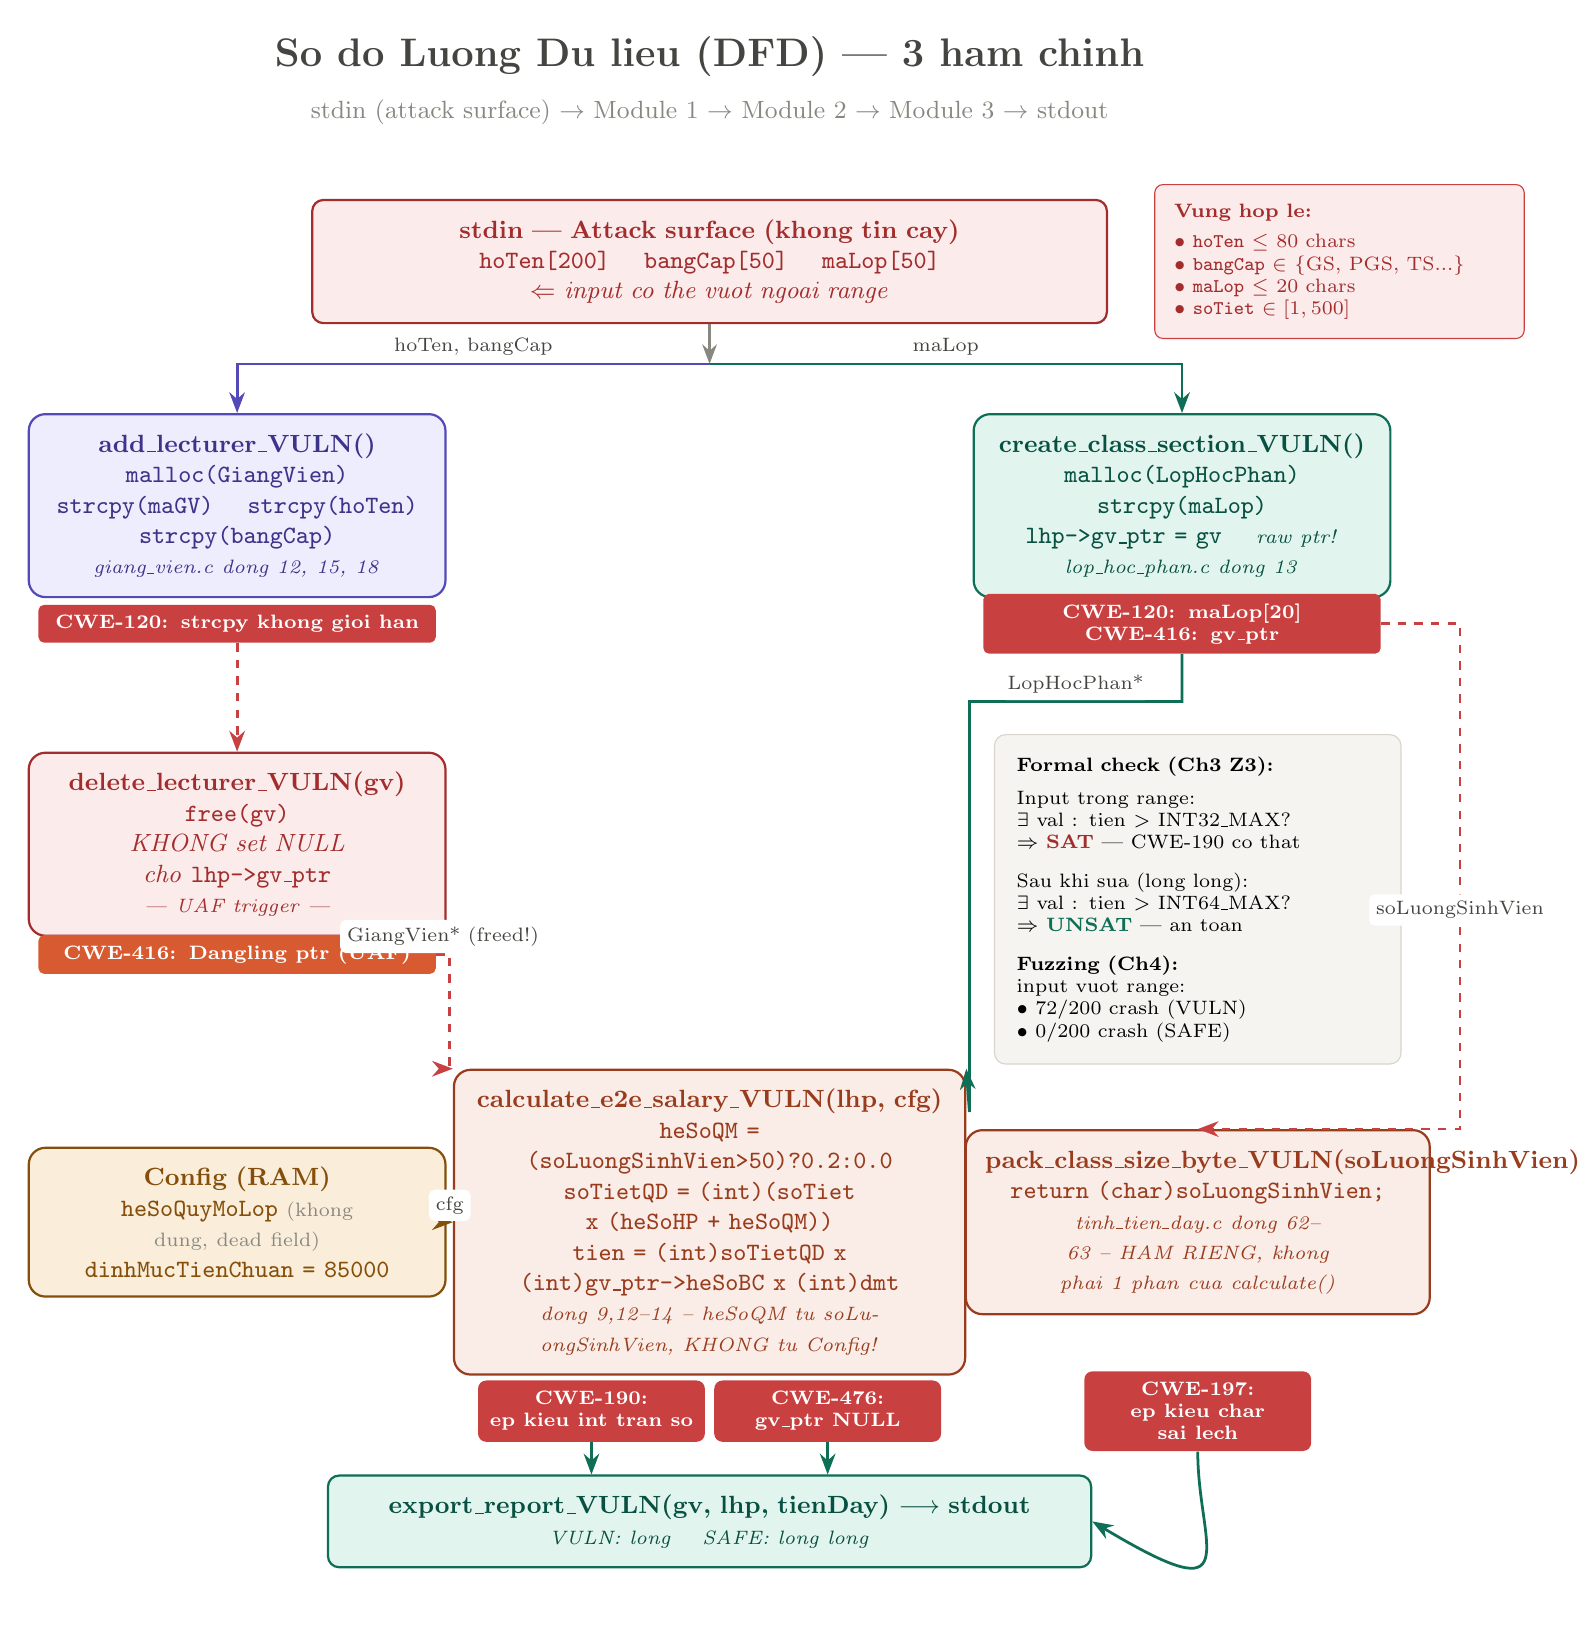
\begin{tikzpicture}

%% ===== TITLE =====
\node[title main] (T3) at (0, 8.2)
  {So do Luong Du lieu (DFD) --- 3 ham chinh};
\node[title sub] (T3sub) at (0, 7.5)
  {stdin (attack surface) $\to$ Module 1 $\to$ Module 2 $\to$ Module 3 $\to$ stdout};

%% ===== ATTACK SURFACE: stdin =====
\node[dfd io, fill=CRed50, draw=CRed600, text=CRed600] (stdin) at (0, 5.6)
{
  \textbf{stdin --- Attack surface (khong tin cay)}\\
  \texttt{\small hoTen[200]} \quad \texttt{bangCap[50]} \quad \texttt{maLop[50]}\\
  $\Leftarrow$ \textit{input co the vuot ngoai range}
};

%% ===== RANGE ANNOTATION =====
\node[draw=CRed400, fill=CRed50, rounded corners=3pt,
  font=\scriptsize, text=CRed600,
  inner sep=7pt, text width=4.2cm, align=left] (range note) at (8.0, 5.6)
{
  \textbf{Vung hop le:}\\[3pt]
  $\bullet$ \texttt{hoTen} $\leq$ 80 chars\\
  $\bullet$ \texttt{bangCap} $\in$ \{GS, PGS, TS...\}\\
  $\bullet$ \texttt{maLop} $\leq$ 20 chars\\
  $\bullet$ \texttt{soTiet} $\in [1, 500]$
};

%% ===== LEVEL 1: MODULE 1 & MODULE 2 =====
%% add_lecturer_VULN()
\node[dfd process, fill=CPurple50, draw=CPurple600, text=CPurple800] (add lec) at (-6.0, 2.5)
{
  \textbf{add\_lecturer\_VULN()}\\
  \texttt{\small malloc(GiangVien)}\\
  \texttt{\small strcpy(maGV)} \quad \texttt{\small strcpy(hoTen)}\\
  \texttt{\small strcpy(bangCap)}\\
  \textit{\scriptsize giang\_vien.c dong 12, 15, 18}
};

\node[badge, fill=CRed400, text width=4.8cm, align=center] (cwe add) at (-6.0, 1.0)
  {CWE-120: strcpy khong gioi han};

%% create_class_section_VULN()
\node[dfd process, fill=CTeal50, draw=CTeal600, text=CTeal800] (create cls) at (6.0, 2.5)
{
  \textbf{create\_class\_section\_VULN()}\\
  \texttt{\small malloc(LopHocPhan)}\\
  \texttt{\small strcpy(maLop)}\\
  \texttt{\small lhp->gv\_ptr = gv} \quad \textit{\scriptsize raw ptr!}\\
  \textit{\scriptsize lop\_hoc\_phan.c dong 13}
};

\node[badge, fill=CRed400, text width=4.8cm, align=center] (cwe cls) at (6.0, 1.0)
  {CWE-120: maLop[20] \quad CWE-416: gv\_ptr};

%% Split arrows from stdin to add_lecturer and create_class_section
\coordinate (split) at (0, 4.3);
\draw[arr] (stdin.south) -- (split);
\draw[arr purple] (split) -- node[edge label, above, midway] {hoTen, bangCap} (-6.0, 4.3) -- (add lec.north);
\draw[arr teal]   (split) -- node[edge label, above, midway] {maLop} (6.0, 4.3) -- (create cls.north);

%% ===== LEVEL 2: DELETE LECTURER & FORMAL BOX =====
%% delete_lecturer_VULN()
\node[dfd process, fill=CRed50, draw=CRed600, text=CRed600] (del lec) at (-6.0, -1.8)
{
  \textbf{delete\_lecturer\_VULN(gv)}\\
  \texttt{\small free(gv)}\\
  \textit{KHONG set NULL cho} \texttt{\small lhp->gv\_ptr}\\
  \textit{\scriptsize --- UAF trigger ---}
};

\node[badge, fill=CCoral400, text width=4.8cm, align=center] (cwe del) at (-6.0, -3.2)
  {CWE-416: Dangling ptr (UAF)};

\draw[arr red] (cwe add.south) -- (del lec.north);

%% Formal check & Fuzzing box (Right Column)
\node[draw=CGray200, fill=CGray50, rounded corners=4pt,
  font=\scriptsize, inner sep=8pt,
  text width=4.6cm, align=left] (formal box) at (6.2, -2.5)
{
  \textbf{Formal check (Ch3 Z3):}\\[4pt]
  Input trong range:\\
  $\exists$ val : tien $>$ INT32\_MAX?\\
  $\Rightarrow$ \textcolor{CRed600}{\textbf{SAT}} --- CWE-190 co that\\[6pt]
  Sau khi sua (long long):\\
  $\exists$ val : tien $>$ INT64\_MAX?\\
  $\Rightarrow$ \textcolor{CTeal600}{\textbf{UNSAT}} --- an toan\\[6pt]
  \textbf{Fuzzing (Ch4):}\\
  input vuot range:\\
  $\bullet$ 72/200 crash (VULN)\\
  $\bullet$ 0/200 crash (SAFE)
};

%% ===== LEVEL 3: CONFIG & CALCULATE =====
%% Config (RAM)
\node[dfd process, fill=CAmber50, draw=CAmber600, text=CAmber600] (config) at (-6.0, -6.6)
{
  \textbf{Config (RAM)}\\
  \texttt{\small heSoQuyMoLop} \textcolor{CGray500}{\scriptsize (khong dung, dead field)}\\
  \texttt{\small dinhMucTienChuan = 85000}
};

%% calculate_e2e_salary_VULN() (Center)
\node[dfd process, fill=CCoral50, draw=CCoral600, text=CCoral600,
  text width=6.0cm] (calc) at (0, -6.6)
{
  \textbf{calculate\_e2e\_salary\_VULN(lhp, cfg)}\\
  \texttt{\small heSoQM = (soLuongSinhVien>50)?0.2:0.0}\\
  \texttt{\small soTietQD = (int)(soTiet x (heSoHP + heSoQM))}\\
  \texttt{\small tien = (int)soTietQD x (int)gv\_ptr->heSoBC x (int)dmt}\\
  \textit{\scriptsize dong 9,12--14 -- heSoQM tu soLuongSinhVien, KHONG tu Config!}
};

\node[dfd cwe, fill=CRed400, text=CWhite, text width=2.6cm] (cwe190) at (-1.5, -9.0)
  {CWE-190:\\ep kieu int tran so};
\node[dfd cwe, fill=CRed400, text=CWhite, text width=2.6cm] (cwe476) at (1.5, -9.0)
  {CWE-476:\\gv\_ptr NULL};

%% pack_class_size_byte_VULN() -- ham RIENG (khong phai calculate()), dung soLuongSinhVien
%% de dong goi audit log, doc lap voi cong thuc tinh luong o tren
\node[dfd process, fill=CCoral50, draw=CCoral600, text=CCoral600,
  text width=5.4cm] (pack) at (6.2, -6.6)
{
  \textbf{pack\_class\_size\_byte\_VULN(soLuongSinhVien)}\\
  \texttt{\small return (char)soLuongSinhVien;}\\
  \textit{\scriptsize tinh\_tien\_day.c dong 62--63 -- HAM RIENG, khong phai 1 phan cua calculate()}
};
\node[dfd cwe, fill=CRed400, text=CWhite, text width=2.6cm] (cwe197) at (6.2, -9.0)
  {CWE-197:\\ep kieu char sai lech};
\draw[arr red] (cwe cls.east) -- ++(1.0,0) |- node[edge label, pos=0.3, above] {soLuongSinhVien} (pack.north);

%% ===== CONNECTING ARROWS TO CALCULATE =====
%% From delete_lecturer to calculate
\draw[arr red]
  (cwe del.east) -- node[edge label, above] {GiangVien* (freed!)} (-3.3, -3.2) |- (calc.north west);

%% From Config to calculate
\draw[arr amber]
  (config.east) -- node[edge label, above] {cfg} (calc.west);

%% From create_class_section to calculate (routed down the corridor)
\draw[arr teal]
  (cwe cls.south) -- ++(0, -0.6) -| node[edge label, above, pos=0.25] {LopHocPhan*} (3.3, -5.2) -- (calc.north east);

%% ===== LEVEL 4: OUTPUT =====
\node[dfd io, fill=CTeal50, draw=CTeal600, text=CTeal800,
  text width=9.2cm] (export) at (0, -10.4)
{
  \textbf{export\_report\_VULN(gv, lhp, tienDay)} $\longrightarrow$ \textbf{stdout}\\
  \textit{\scriptsize VULN: long \quad SAFE: long long}
};

\draw[arr teal] (cwe190.south) -- (cwe190.south |- export.north);
\draw[arr teal] (cwe476.south) -- (cwe476.south |- export.north);
\draw[arr teal] (cwe197.south) .. controls +(0,-1.2) and +(2,-1.2) .. (export.east);

\end{tikzpicture}
\end{document}
